\chapter{The Basics}
\chapteroverlay
\section{File states}
Git has three main states that your files can reside in: \textit{modified}, \textit{staged}, and \textit{committed}:
\begin{enumerate}
    \item \textbf{Modified} means that you have changed the file but have not committed it to your database yet.
    \item \textbf{Staged} means that you have marked a modified file in its current version to go into your next commit snapshot.
    \item \textbf{Committed} means that the data is safely stored in your local database.
\end{enumerate}

\begin{figure}[H]
\centering
    \centering
    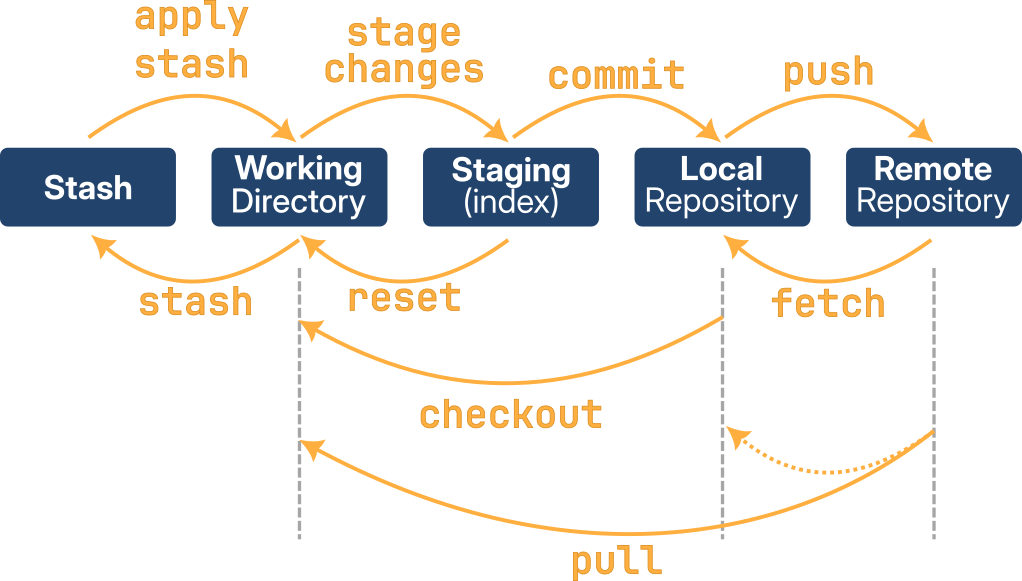
\includegraphics[scale=1]{Images/recordingChanges.png}
    \caption{recording Changes}
\end{figure}
    
\subsection{Lifecycle of file statuses}
Each file in your working directory can be in one of two states: \textbf{tracked} or \textbf{untracked}. Tracked files are files that Git is aware of and were either in the last snapshot\footnotemark or are newly staged files.
Tracked files can be \textit{unmodified}, \textit{modified}, or \textit{staged}. \newline
While git knows about all files in your working directory, it will only \textit{watch} and record the history of \textbf{tracked} files.

\begin{figure}[H]
\centering
    \centering
    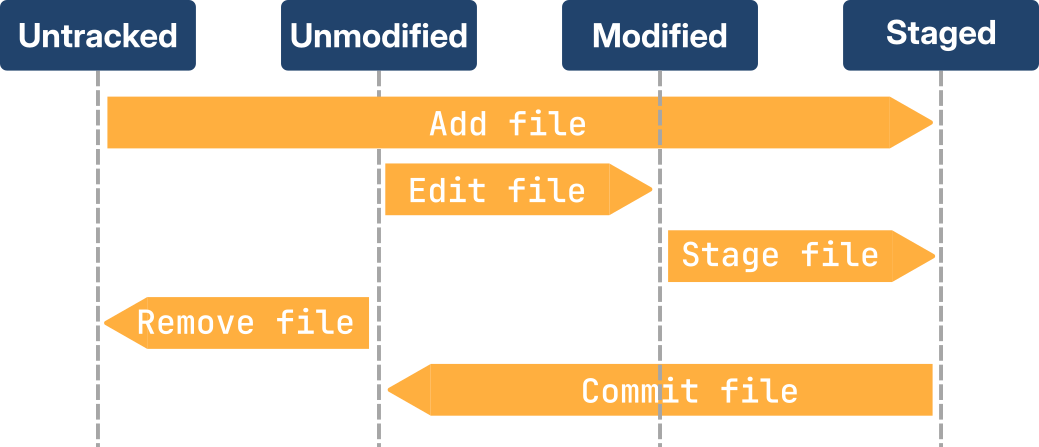
\includegraphics[scale=1]{Images/workingTree.png}
    \caption{Working tree}
\end{figure}

\section{Commit Lifecycle}
The commit lifecycle begins by checking the state of files, then adding the desired files to the staging area, and finally committing them to the repository. Commits can also be pushed to a remote repository.

\subsection{File States}
To check the states of our files we can use:
\begin{gitBashBox}
status
\end{gitBashBox}
\noindent Adding the \textit{short} flag\footnotemark gives a more concise output, if the regular one is too long. The \gitinline{status -s} and \gitinline{tsatus --short} syntax are synonymous to one another.
\begin{table}[H]
    \centering
    \begin{tabular}{c|l}
       \hspace{2mm} M  & modified but not staged\\[2pt]
       M\hspace{3mm}   & modified and staged\\[2pt]
       MM  & modified, staged and then modified again \\[2pt]
       A\hspace{3mm}   & new files added to staging area \\[2pt]
       ?\hspace{0.7mm}?  & new files that aren't tracked \\
       
    \end{tabular}
    \caption{Shorthand symbol meaning}
    \label{tab:short_symbols}
\end{table}

\noindent If \textit{git status} is too vague, use \gitinline{git diff} it shows changes between your working directory and the staging area. \textbf{→ unstaged changes}\newline
\gitinline{git diff --staged} and \gitinline{git diff --cached}\hspace{1mm}\footnotemark\hspace{0.2mm} will shows changes between the staging area and the last commit.  \textbf{→ staged changes}

If you have a newly untracked directory with a bunch of untracked files \gitinline{git diff} will only show you the untracked directory, not all the files inside that aren't tracked either. To see these you can \gitinline{dit diff -uall}, which is short for \gitinline{git diff --untracked-files=all}.
\subsection{Tracking and Staging}
\noindent Track and stage new files using:
\begin{gitBashBox}
add <file>
\end{gitBashBox}
\noindent The git add command takes a path name for either a file or a directory; if it’s a directory, the command adds all the files in that directory recursively.

\subsection{Committing staged changes}
When the staging area is set up the way you want it, you can commit your changes with \gitinline{git commit}. This will however open a text editor for you to enter your commit message and if using the \gitinline{-v} verbose tag, will display more information on what will be commited.\newline
Becasue we are lazy we can use:
\begin{gitBashBox}
commit -m "message"
\end{gitBashBox}
This allows us to skip the editor step and type up our comment in the editor itself.\newline

If you want to skip the staging are, one can add the \gitinline{-a} flag. This will  also add all tracked files.

\section{undo mistaken commit}
1. Undo last commit but keep changes staged
\begin{gitBashBox}
git reset --soft HEAD~1
\end{gitBashBox}

2. Undo last commit and unstage changes
\begin{gitBashBox}
git reset --mixed HEAD~1
\end{gitBashBox}

3. Undo last commit and discard changes
\begin{gitBashBox}
git reset --hard HEAD~1
\end{gitBashBox}

\subsection{Undo when pushed}
\begin{gitBashBox}
revert <commit>
\end{gitBashBox}
Where <commit> is the commit hash.
Use \gitinline{git log} or \gitinline{git log --oneline}.
\gitinline{git --no-pager log} doesn't leave you in the pager, which you would normally equit with \textbf{q}.


% --- Footnotes ---
\footnotetext{A Snapshot is your last commit, see Glossary for more details.}
\footnotetext{A flag is a parameter you pass to a Git command to modify its behavior. There are short (-s) and long (-\hspace{0.1mm}-short) flags. Functionally \textit{most} Git commands treats them the same.}
\footnotetext{-\hspace{0.1mm}-chaced is older terminology}